\chapter{Implementation, Integration and Test Plan}
\section{Implementation plan}
Motivated by effectiveness of the agile approach as opposed to the traditional ones, the development of the DREAM system is organized in an iterative way \cite{agile}. The stakeholders should assist throughout the whole development process, providing relevant feedback. The goal is to quickly provide the Minimum Viable Product (MVP) that has just enough functionality to satisfy the users and collect feedback for further development as soon as possible \cite{mvp}.

In order to break down the implementation into iterative phases, a list of dependencies between the components was created:
\begin{longtable}{@{}p{0.06\linewidth} p{0.90\linewidth}@{}}
    \autonum{D} &  The Business Layer components' implementation requires prior implementation of Data Access Layer to provide persistence of data. \\
    
    \autonum{D} &  The implementation of  \textit{AccountController} and \textit{AccountService} requires prior implementation of \textit{EmailSender} to provide the functionality of sending reset password e-mails.\\
    
    \autonum{D} &  The implementation of all \textit{controller}s and dependent services requires prior implementation of \textit{AccountController} and \textit{AccountService} to provide the authorization mechanisms required by the HTTP endpoints defined by the \textit{controller}s.\\
    
    \autonum{D} &  The implementation of \textit{AgronomistController} and \textit{AgronomistService} requires prior implementation of \textit{VisitsPlanner} to provide the implementation of Visit Scheduling Algorithm (\ref{subsec:visits-alg}) that ensures each farm is visited at least twice a year.\\
    
    \autonum{D} &  The implementation of \textit{FarmerController} and \textit{FarmerService} requires prior implementation of \textit{VisitsPlanner} to provide the implementation of Visit Scheduling Algorithm (\ref{subsec:visits-alg}) that ensures each farm is visited more frequently if a farmer has obtained a negative note.\\
    
    \autonum{D} &  Optional:  The implementation of \textit{FarmerController} and \textit{FarmService} as well as 
    \textit{WeatherForecastController} and \textit{WeatherForecastrService}
    requires prior implementation of \textit{ExternalSystemsReader} to ensure that database contains data from external systems to be read by dependent components. However, this dependency can be relaxed either by accepting empty values returned by the API or by providing some static data.\\
\end{longtable}

All components not mentioned above can be built in any sequence. However, a specific implementation order, which favors the delivery of users' most  valued functionalities first, is proposed in the following part of the document.

The implementation of the Web Application views presented in the chapter \ref{chap:ui} is achieved in an iterative way, by the creation of the views corresponding to the DREAM Server Application functionalities developed in the given iteration. However, the views can be developed independently since the communication with the DREAM Server Application can be mocked. 

The first development phase will focus on the Data Access Layer of the DREAM Server Application as well ass the components required for users' registration and log in to address the dependencies \textbf{D1}, \textbf{D2}, and \textbf{D3}. The components built in this step are presented in the figure \ref{fig:step1}. In case of any issues, the first phase can be further broken down into two phases, with the first part containing only the Data Access components.

\begin{figure}[H]
    \centering
    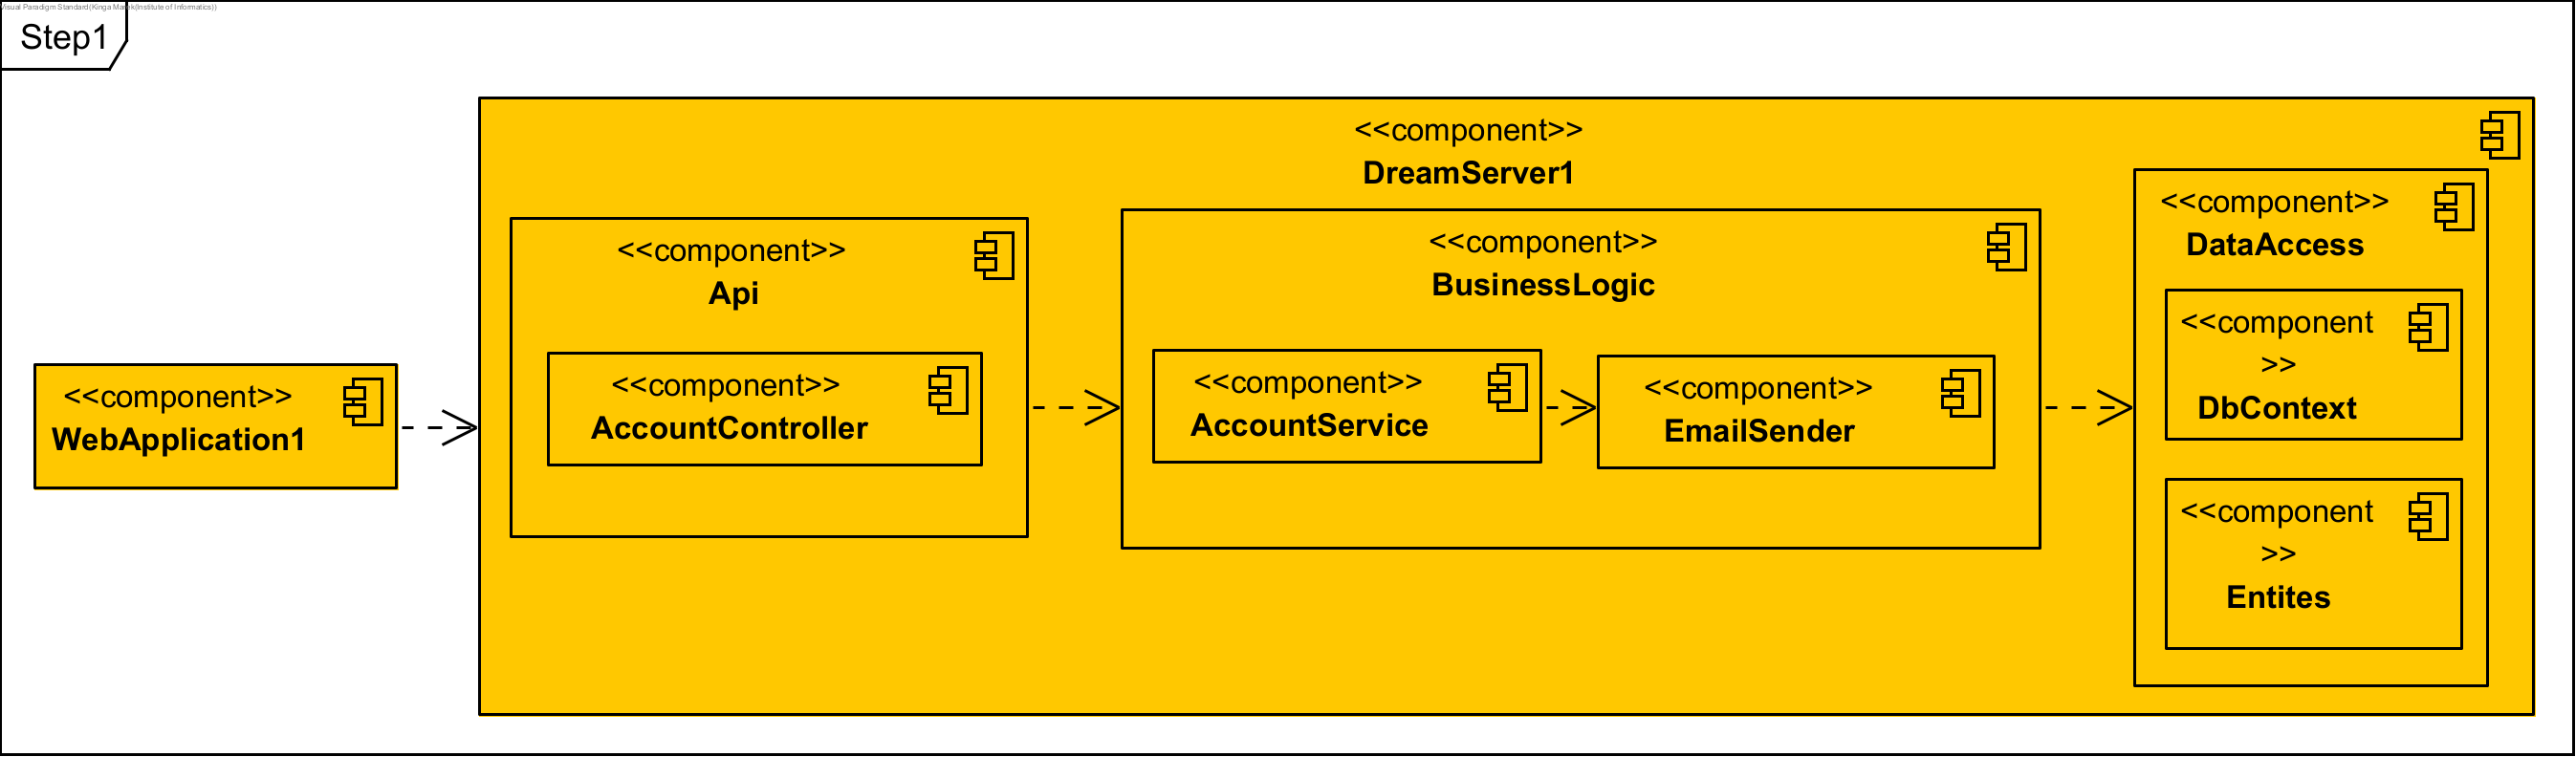
\includegraphics[width=\textwidth]
    {diagrams/implementation-plan/Step1.png}
    \caption{Step 1 of the implementation plan. Components added in this step are highlighted with orange color.}
    \label{fig:step1}
\end{figure}

The second step of the development is presented in the figure \ref{fig:step2}. The focus of this stage is on delivery of the first functionality available for the farmers after registration in the system. Those farmers will be able to exchange knowledge using the forum.  Afterwards, the first MVP for the farmers' can be released. Additionally, this phase aims at providing \textit{VisitsPlanner} to allow the implementation of \textit{AgronomistController} and \textit{AgronomistService} in the following one (resolving the dependency \textbf{D4}). Furthermore, the introduction of requests for help functionality is started by development of \textit{RequestService}.

\begin{figure}[H]
    \centering
    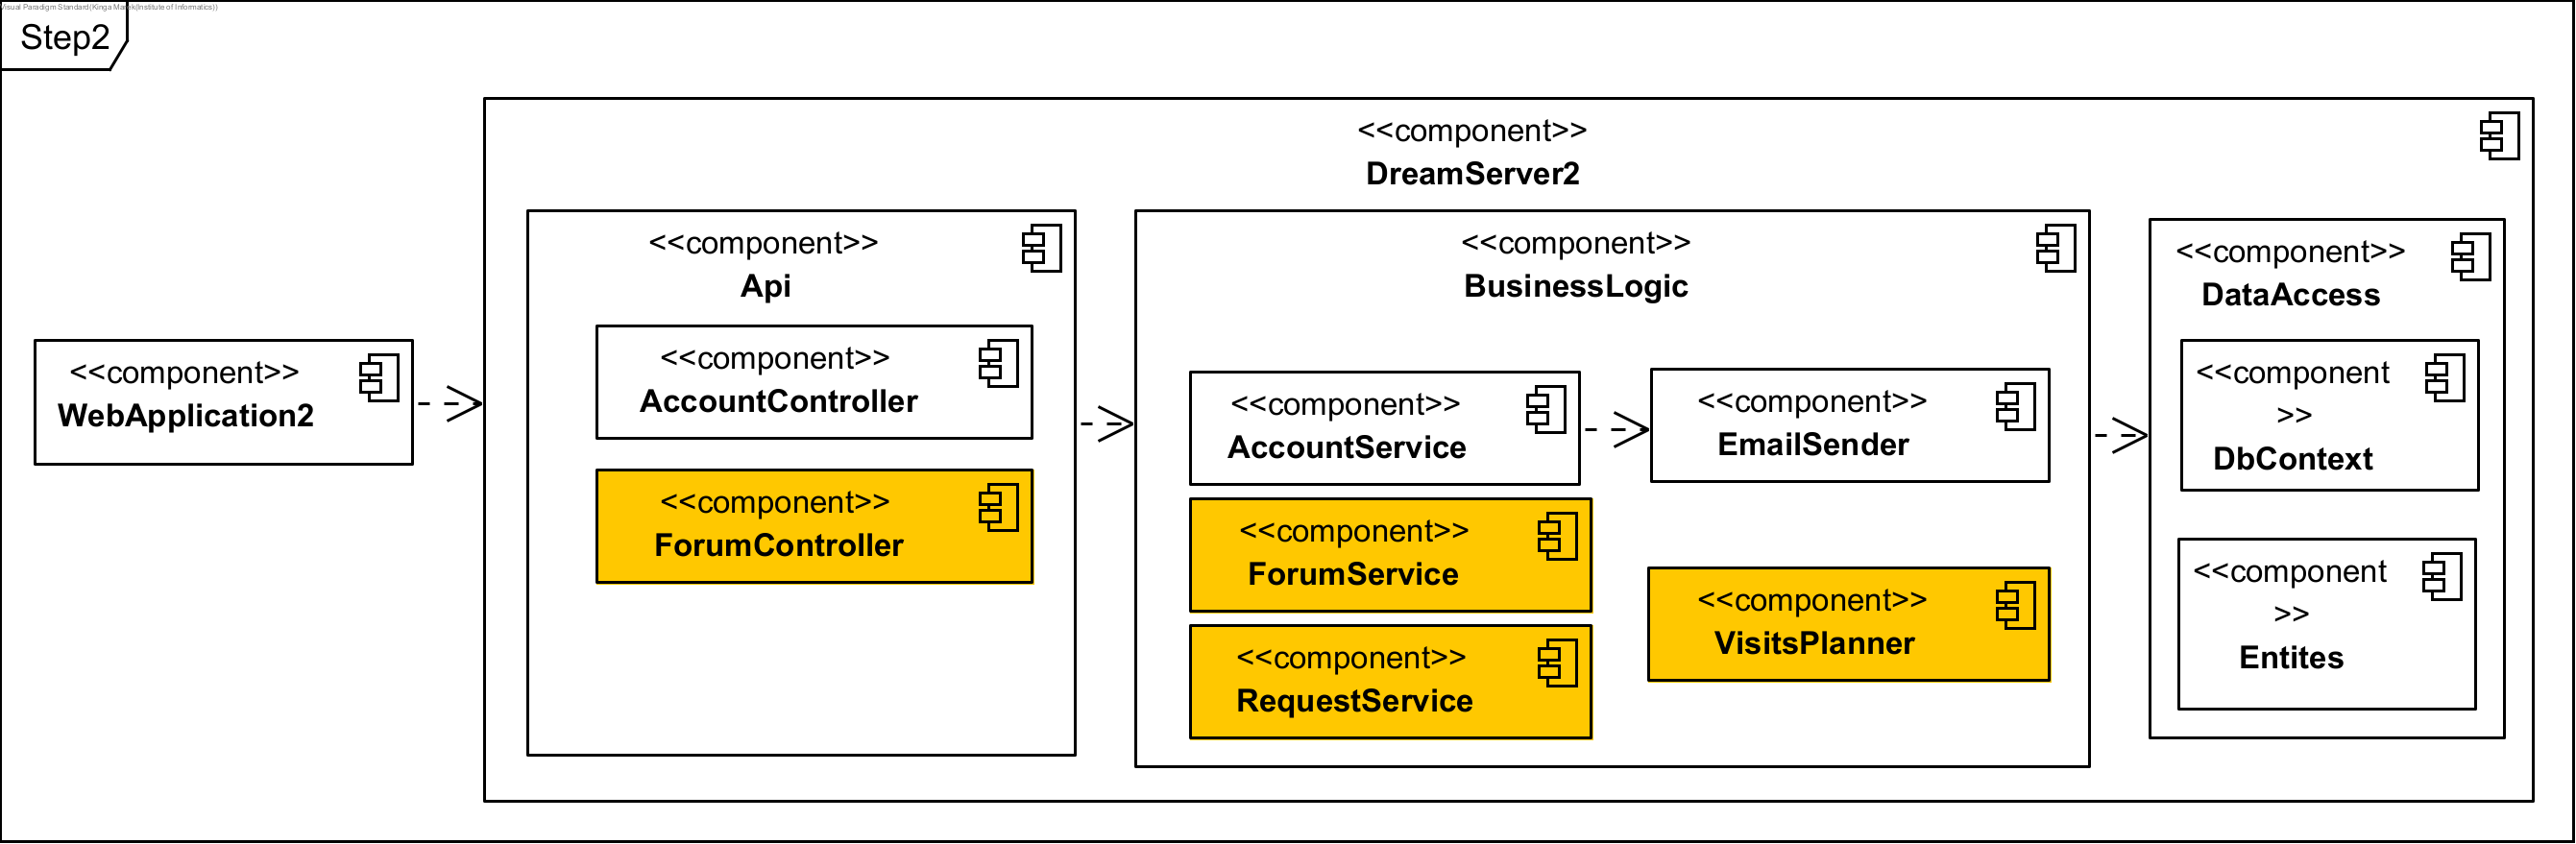
\includegraphics[width=\textwidth]
    {diagrams/implementation-plan/Step2.png}
    \caption{Step 2 of the implementation plan. Components added in this step are highlighted with orange color.}
    \label{fig:step2}
\end{figure}

Thereafter, the third phase presented in the figure \ref{fig:step3} is focused on finishing the requests for help functionality. This part of the system was given a very high importance since it introduces the communication between well-performing and poorly-performing farmers, as well as the agronomists and farmers. From now on, each development phase may be considered as a new MVP release of the product.

Moreover, the agronomists' daily plan functionalities are delivered with the use of previously introduced \textit{VisitsPlanner}.

In addition, the integration with the external systems is started by implementing \textit{WeatherForecastService}.

\begin{figure}[H]
    \centering
    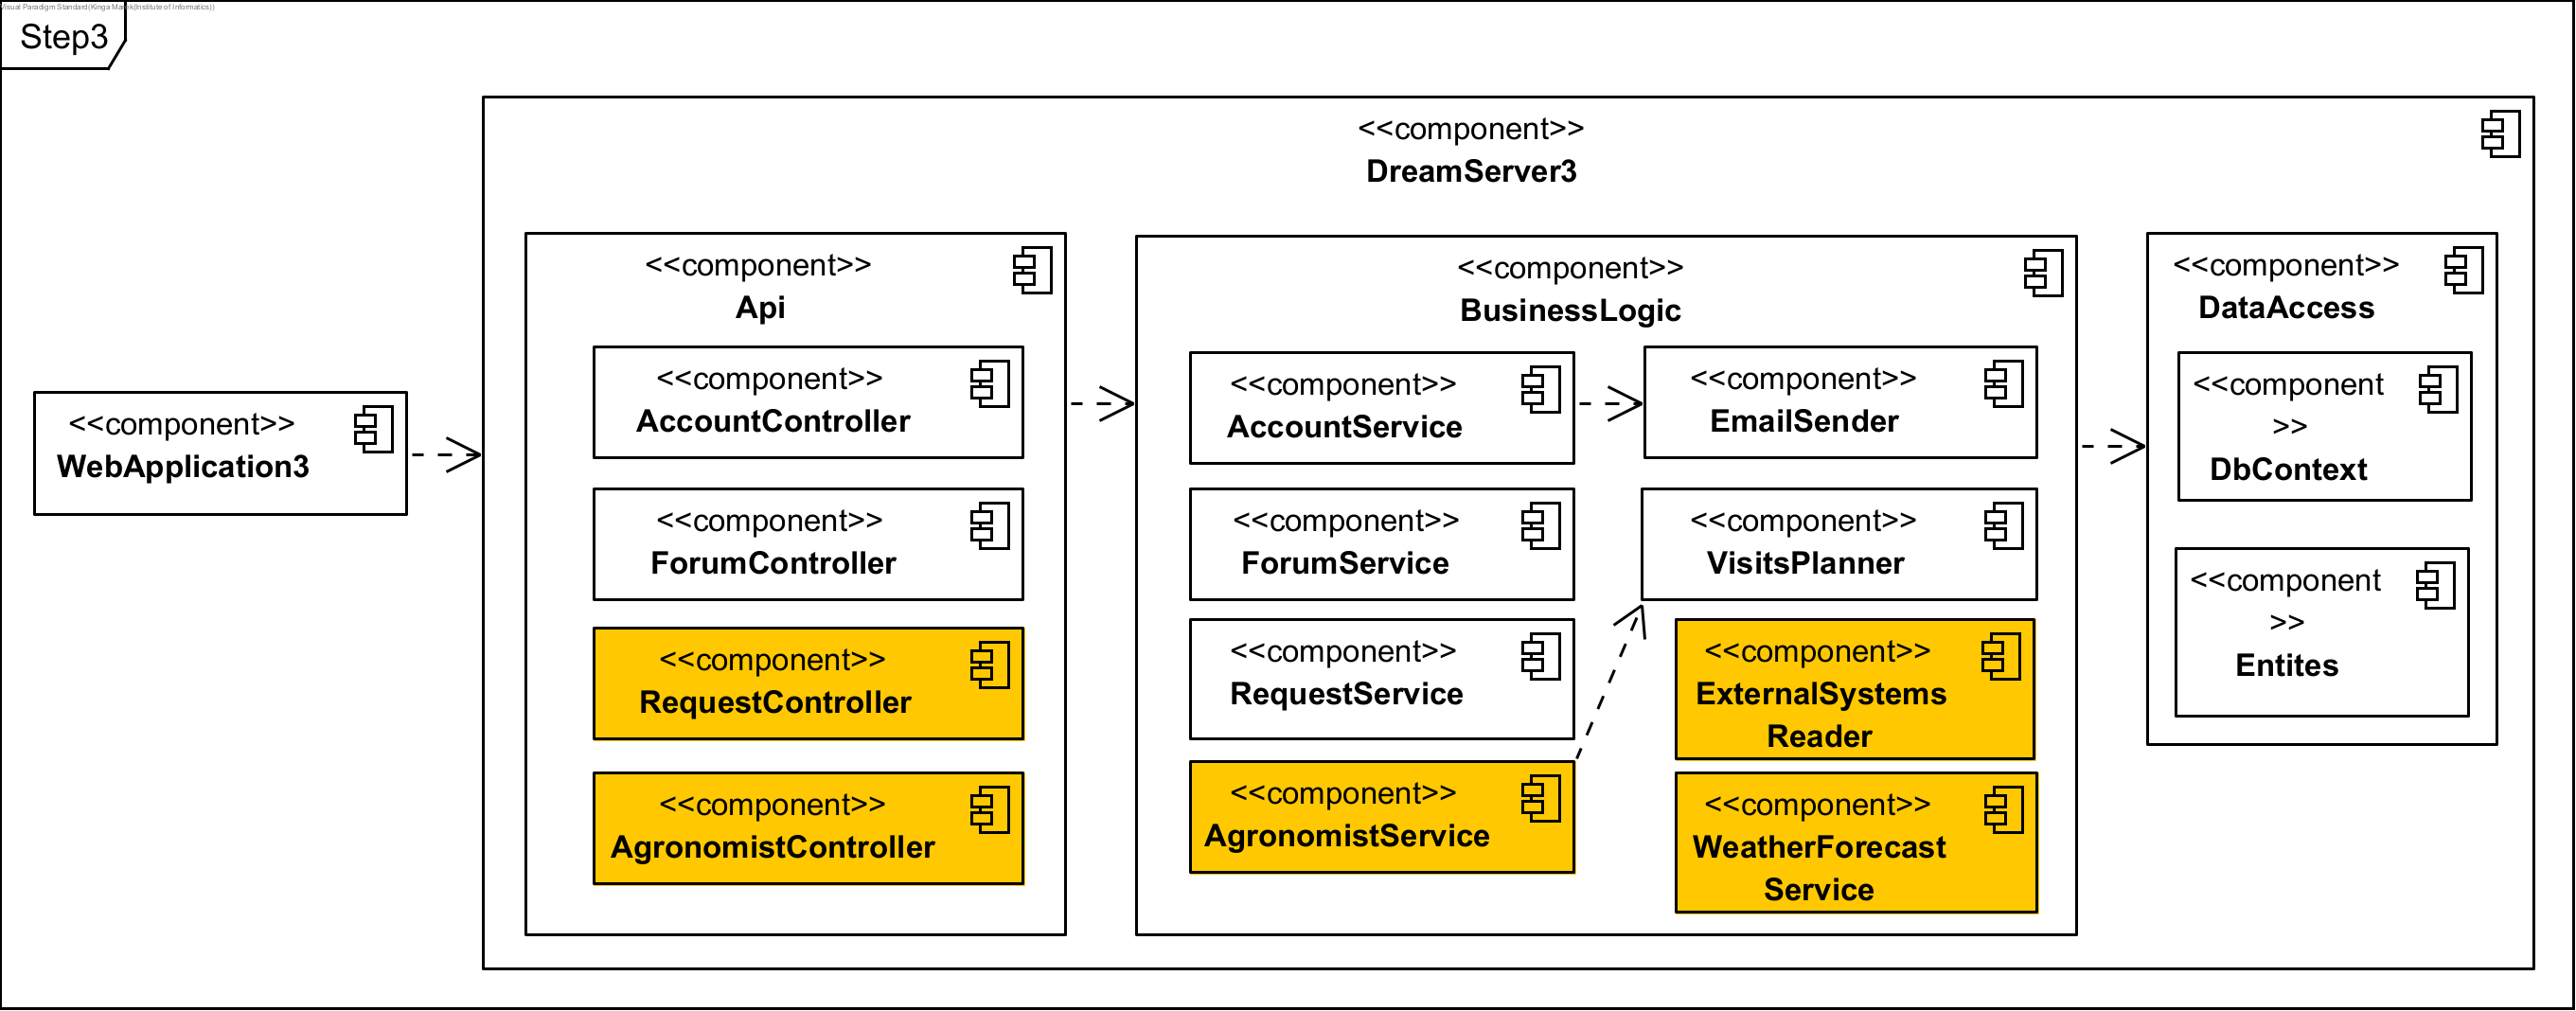
\includegraphics[width=\textwidth]
    {diagrams/implementation-plan/Step3.png}
    \caption{Step 3 of the implementation plan. Components added in this step are highlighted with orange color.}
    \label{fig:step3}
\end{figure}

Step four concentrates on the integration with the external systems' data by introducing the \textit{WeatherForecastController} as well as the \textit{FarmerController}. The former provides information about short and long-term weather forecasts, and the latter delivers data from the farms' irrigation and sensor systems. The information from the external systems will be available in the database thanks to the \textit{ExternalSystemsReader} built in the previous step (\textbf{D6} resolved). The components developed in this phase are presented in the figure \ref{fig:step4}. The implementation of the \textit{FarmerController} can be done since the dependency \textbf{D5} has been resolved in the step 2. Moreover, the farmers may add their production data to the system and agronomists are able to assess the performance of a given farmer.

\begin{figure}[H]
    \centering
    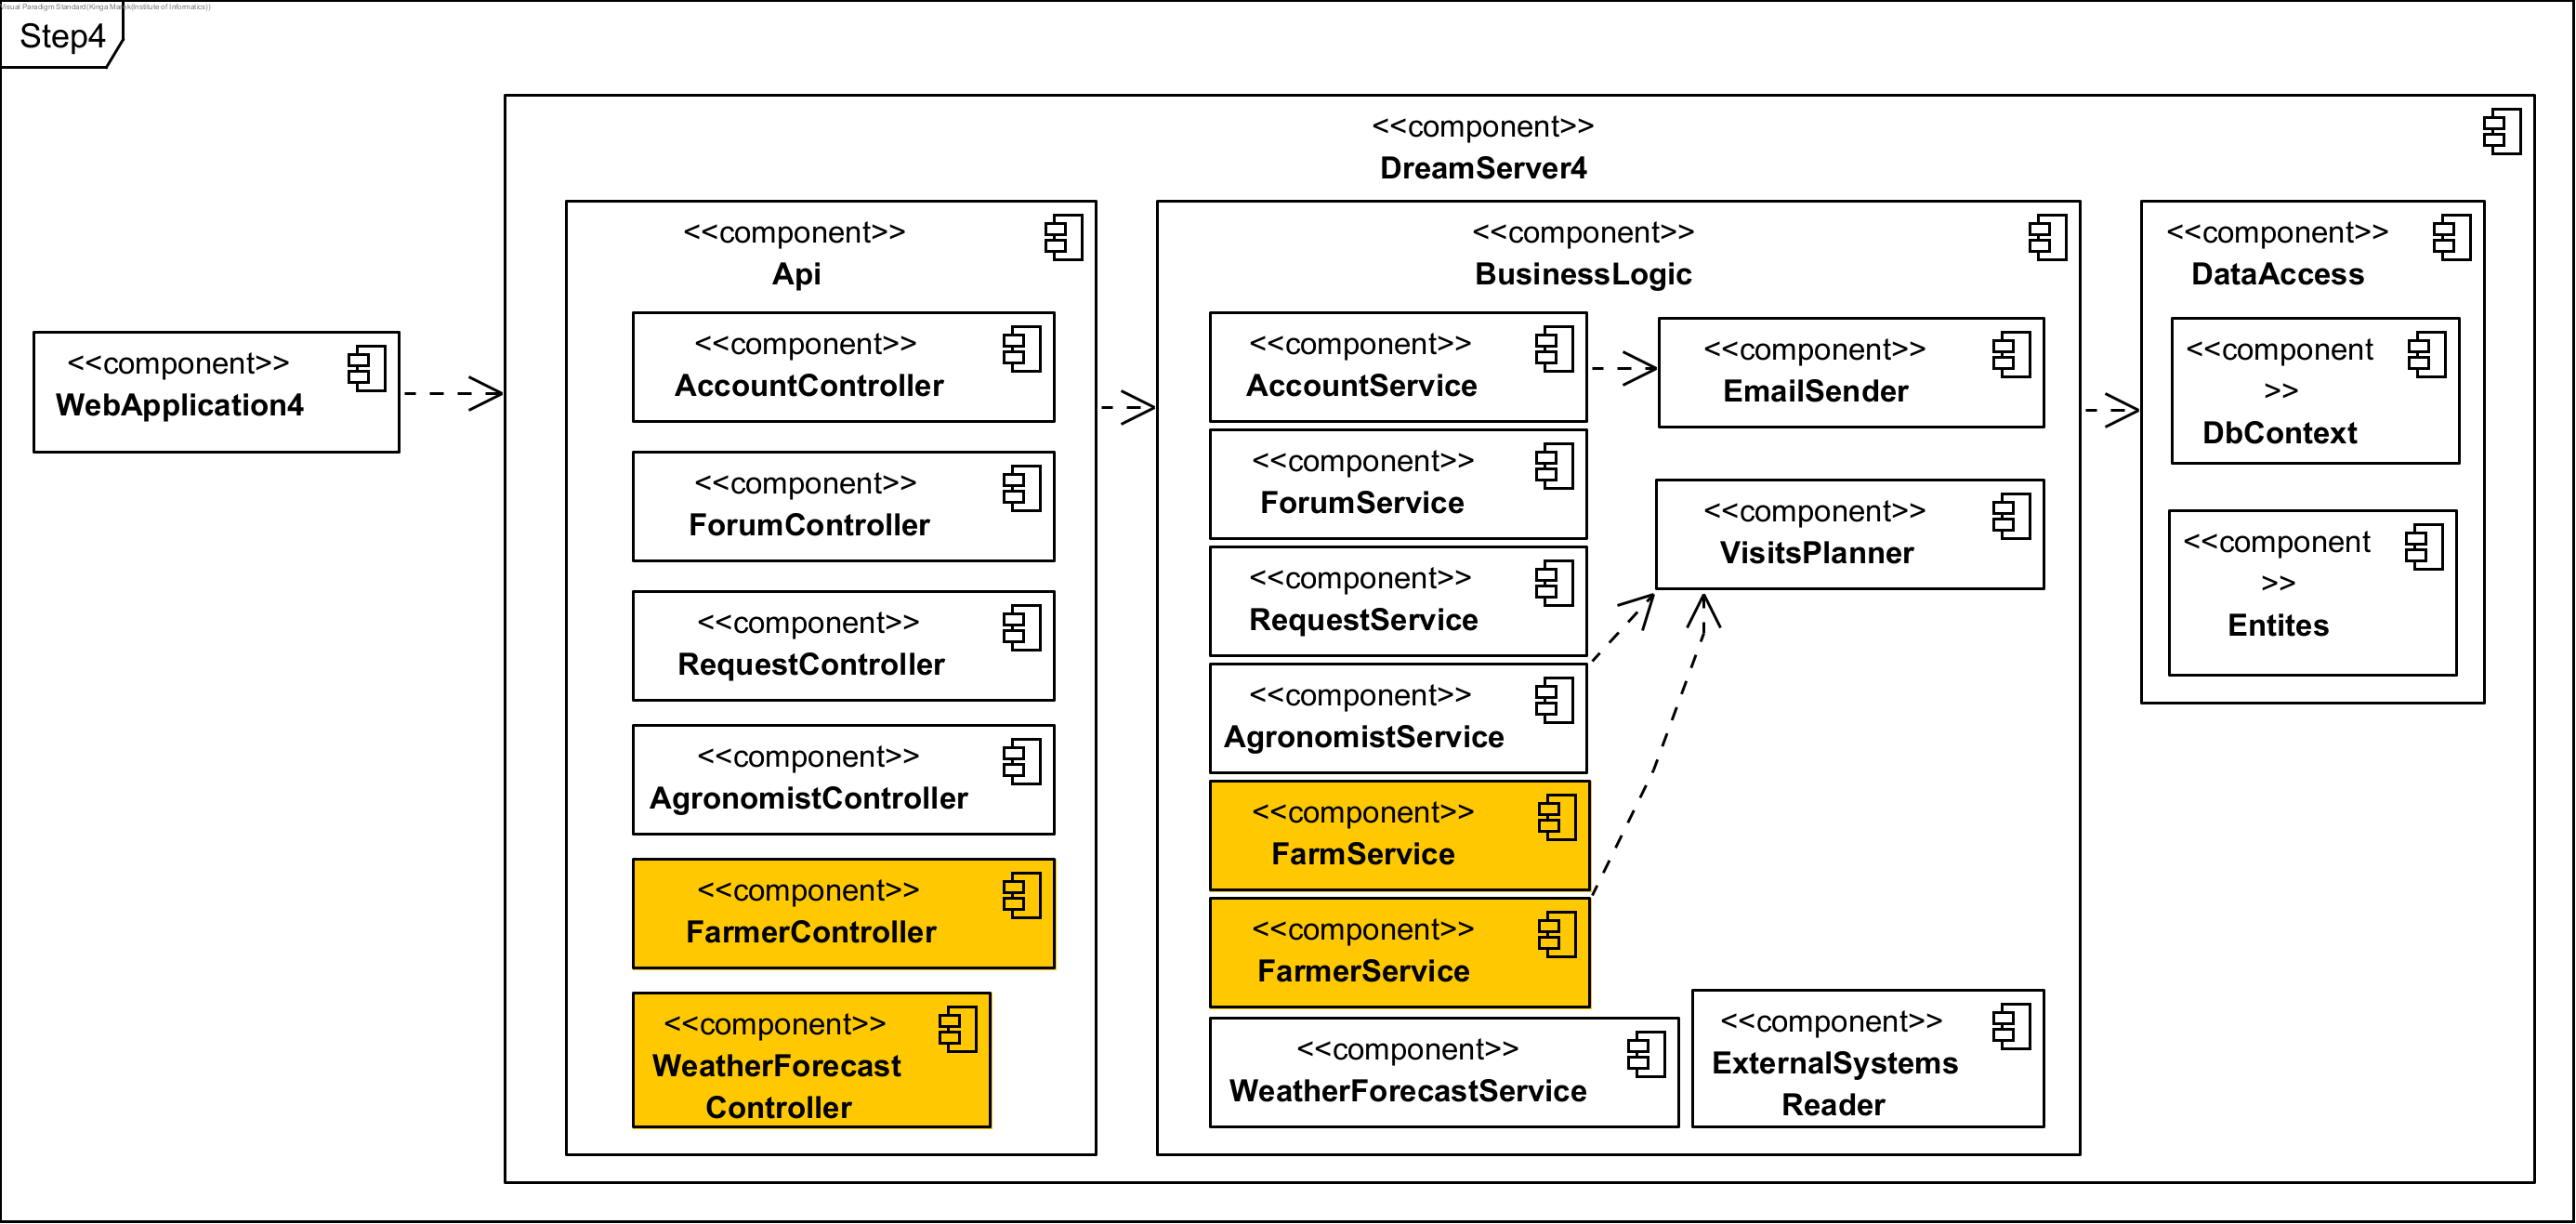
\includegraphics[width=\textwidth]
    {diagrams/implementation-plan/Step4.png}
    \caption{Step 4 of the implementation plan. Components added in this step are highlighted with orange color.}
    \label{fig:step4}
\end{figure}

In the last development phase, the suggestions' functionality is delivered. From now on, the agronomists are able to manage the suggestions for mandals in their area of responsibility. Besides, the system presents personal suggestions for the farmers in their dashboard screen based on the location of their farm and production type. The last implementation step is presented in the figure \ref{fig:step5}.

\begin{figure}[H]
    \centering
    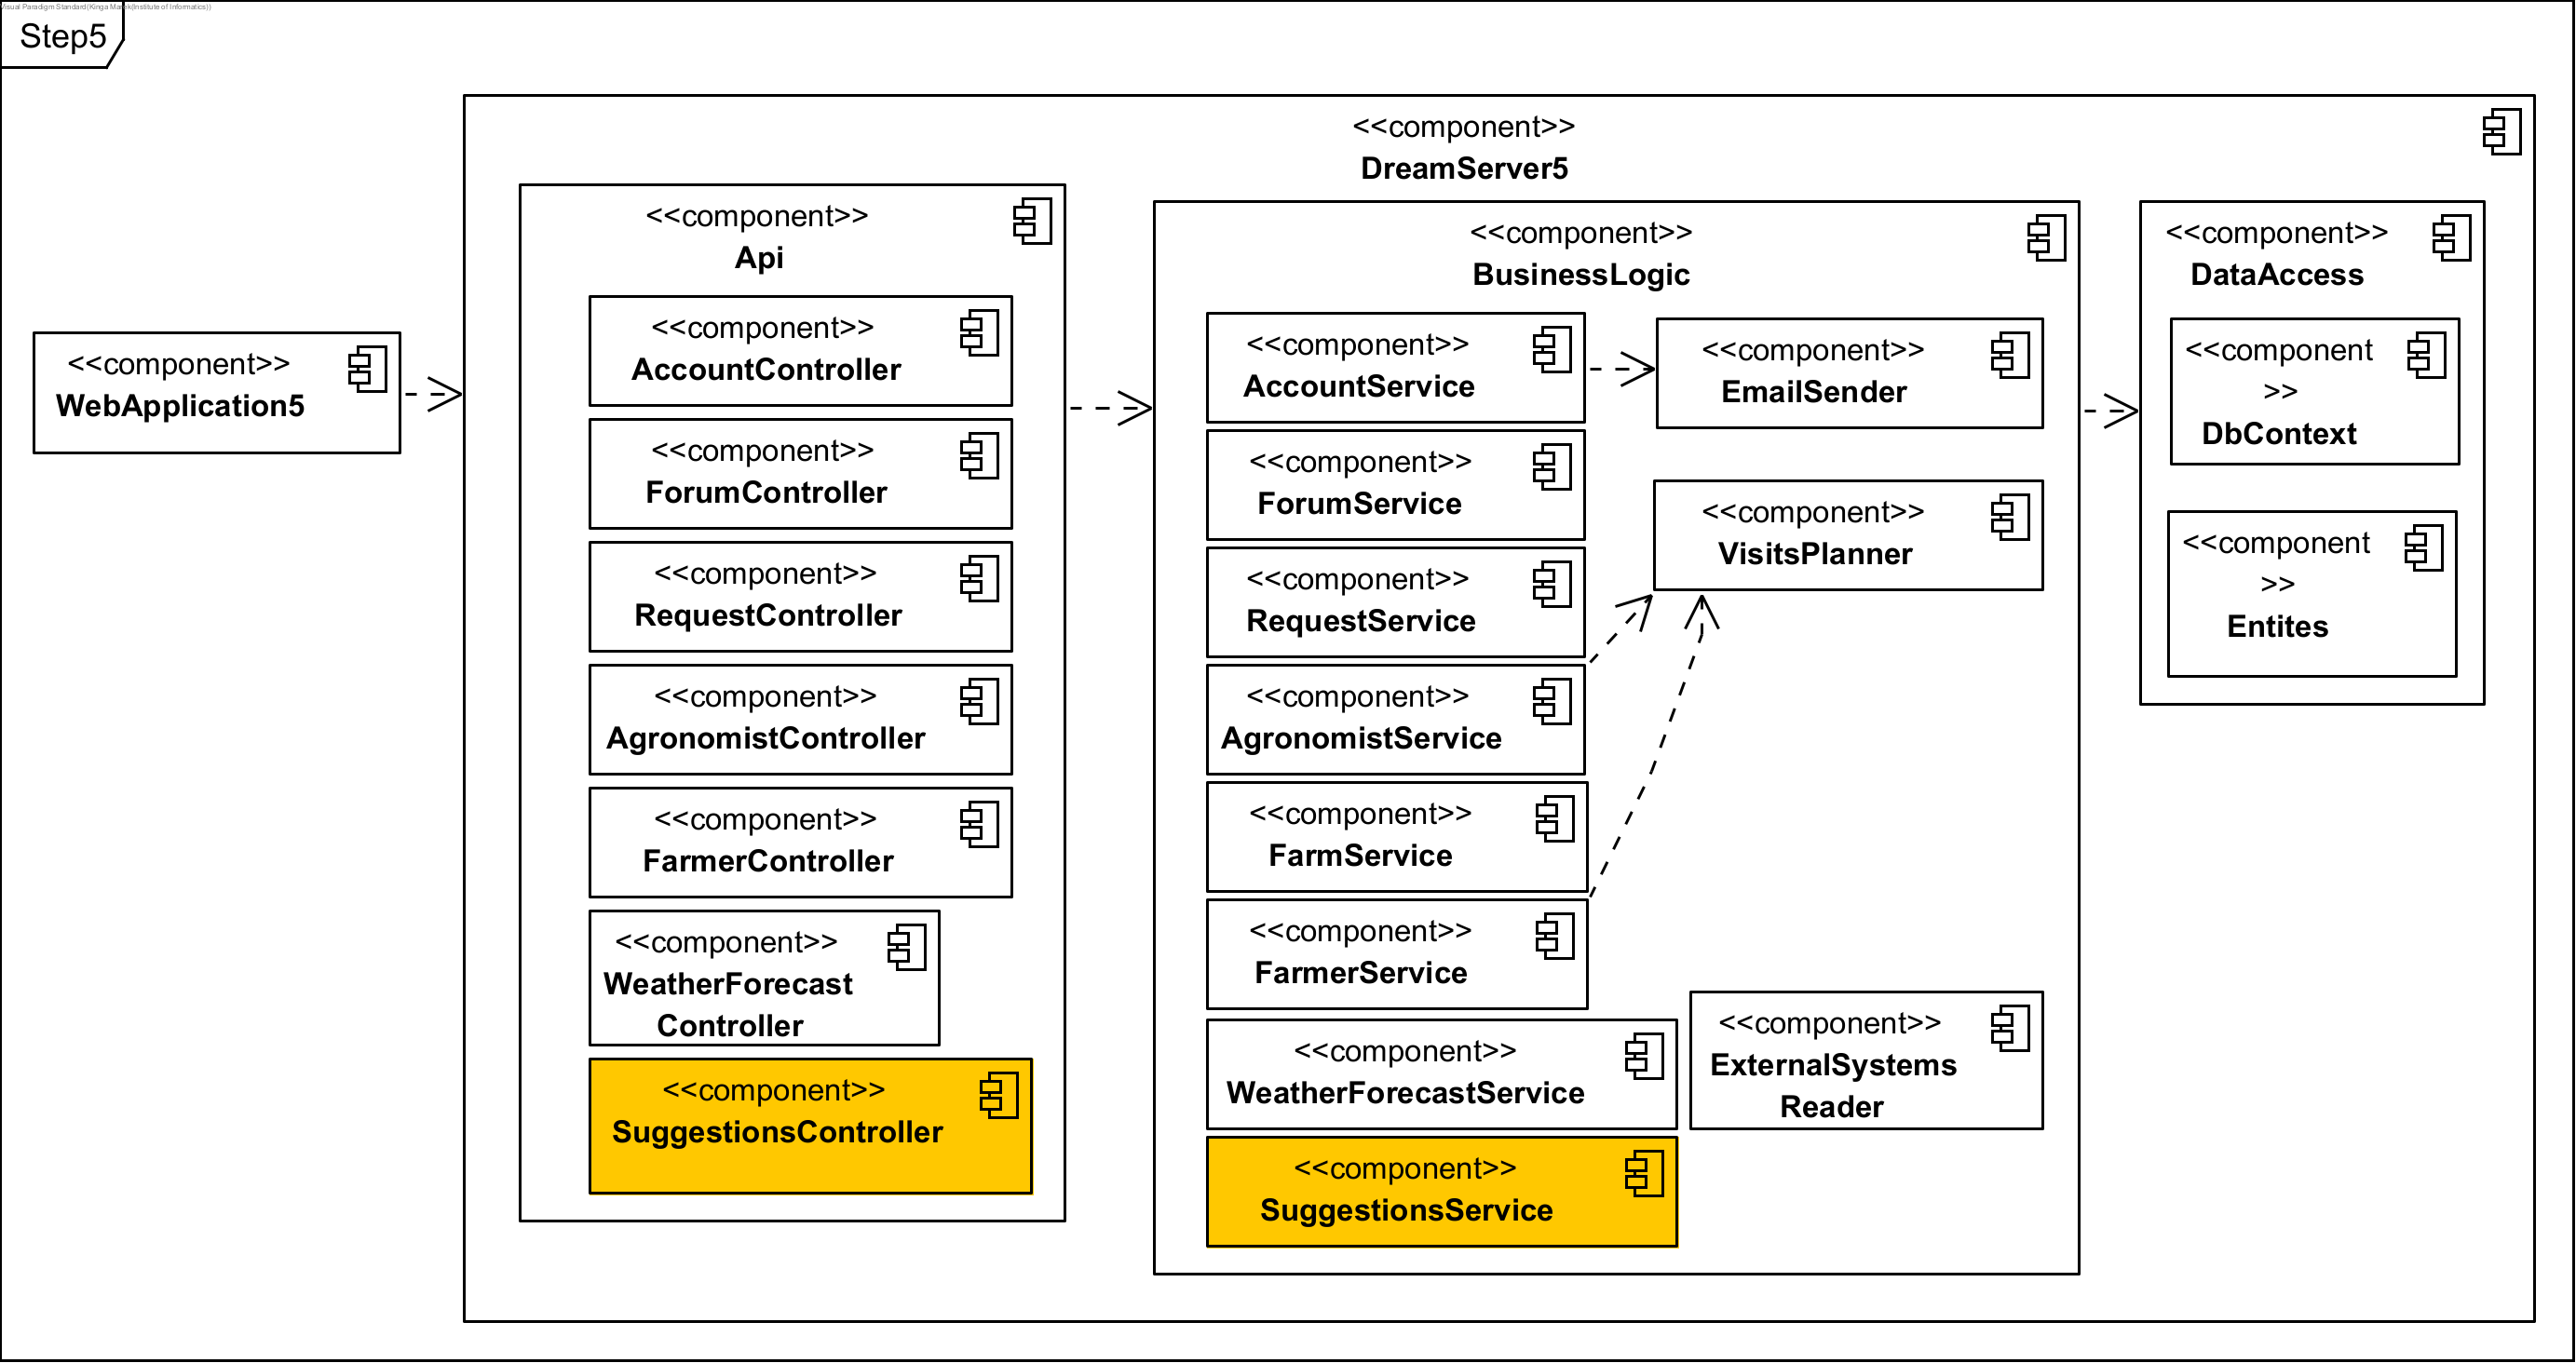
\includegraphics[width=\textwidth]
    {diagrams/implementation-plan/Step5.png}
    \caption{Step 5 of the implementation plan. Components added in this step are highlighted with orange color.}
    \label{fig:step5}
\end{figure}

\section{Integration and test plan}